\documentclass{article}
\usepackage[utf8]{inputenc}
\usepackage{graphicx}
\usepackage[a4paper, total={6in, 9in}]{geometry}
\usepackage{amsmath}
\usepackage{mathtools}
\usepackage{steinmetz}
\usepackage{float}
\DeclarePairedDelimiter\evaluat{.}{\rvert}
\reDeclarePairedDelimiterInnerWrapper\evaluat{nostar}{\mathopen{}#2\mathclose{#3}}
\DeclarePairedDelimiter\abs{\lvert}{\rvert}%
\DeclarePairedDelimiter\norm{\lVert}{\rVert}%
\usepackage{pgfplots}
\usepackage{pst-plot}

 
\title{ELEC344 Assignment 3}
\author{Name: Brendan Lai, Student Number: 19241173}
\date{Due: April 18th, 2021}
  
\begin{document}
\maketitle
  
\tableofcontents


% \begin{figure}[H]
%     \centering
%     \includegraphics[width=0.65\textwidth]{q1c-f1.png}
%     \includegraphics[width=0.65\textwidth]{q1c-f2.png}\\
%     \caption{Waveforms for Q1c}
% \end{figure}
% \begin{center}
%  \begin{tabular}{|c |c c c c c||} 
%  \hline
%   Simulated & $V_L$[V]& $i_L$ [A] & $i_C$ [A] & $V_0$ [V] & $i_{in}$ [A] \\ [0.5ex] 
%  \hline\hline
%  min & -12.01 & 1.13 & -0.0478 & 11.998 & 0 \\
%  \hline
%  max & 36.13 & 1.25 & 0.0446 & 12.001 & 1.253\\
%  \hline
%  average & 12.14 & 1.19 & 0 & 12 & 0.626 \\
%  [1ex] 
%  \hline
% \end{tabular}
% \end{center}
\section{Question 1}
For a permanent magnet DC motor with the following parameters:
\begin{center}
 \begin{tabular}{| c | c | c |} 
 \hline
 Armature resistance: $R_a = 0.3 \Omega$ & Armature inductance: $L_a = 5mH$ & Voltage constant: $k_E = 0.4 \frac{V}{rad/sec}$ \\ 
 \hline
 Torque constant: $k_T = 0.4 \frac{Nm}{A}$ & Total inertia: $J_m = 0.025 kg*m^2$ & Rated torque: $t_{rated} = 5Nm$\\
 \hline
\end{tabular}
\end{center}
\begin{figure}[H]
    \centering
    \includegraphics[width=0.65\textwidth]{q1-1.png}
    \caption{Q1 Circuit}
\end{figure}
Further we also know:
\begin{align*}
    V_a &= i_a R_a + L_a \frac{di_a}{dt}+E_a \mbox{ where } \longrightarrow E_a = K_E\omega_m\\
    \tau_{em} &= \tau_L + B \omega_m + J \frac{d\omega_m}{dt}\mbox{ where } \longrightarrow \tau_{em} = k_T i_a
\end{align*}
\section*{Part a:}
Plot steady state torque-speed characteristic for armature voltages of 120V, 75V, 45V
We want to find $\tau(\omega)$. At steady state we know that all the differential portions of the above characteristics tend to zero and as well that the angular motor speed is 0 since it is idled. Moreover:
\begin{align*}
    V_a &= i_a R_a + E_a\\
    \tau_{em} &= \tau_L = k_T i_a\\
    \mbox{Therefore: } i_a &= \frac{\tau_L}{k_T}\\
    \Longrightarrow V_a &= \frac{\tau_L}{k_T}*R_a + E_a \\
    &= \frac{\tau_L}{k_T}*R_a + k_e\omega_m\\
    \mbox{Therefore: } \tau_L &= \frac{k_T}{R_a}(V_a - k_e \omega_m)\\
    \Longrightarrow \tau_L &= \frac{0.4}{0.3}(V_a - 0.4 \omega_m)
\end{align*}
Lastly, at $\omega_m = 0$: $\tau = (\frac{k_T}{R_a})V_a$ and at $\tau=0$: $\omega_m = \frac{V_a}{k_e}$\\
\begin{figure}[H]
    \centering
    \includegraphics[width=0.65\textwidth]{q1-a.png}
    \caption{Plots of the steady state torque-speed characteristic}
\end{figure}
 
\section*{Part b:}
Calculate the armature voltage required to spin a constant torque load of 4Nm at 1800 RPM\\
Next we want to find $V_a$ where $\tau_L = 4Nm$ and $N_s = 1800rpm$. Thus we know:
\begin{align*}
    \omega_m &= 1800 * (\frac{2\pi}{60}) = 188.4956 [rad/s]\\
    \mbox{Recall that: } V_a &= i_a R_a + E_a = i_a R_a + k_e \omega_m \\
    \tau_{em} &= \tau_L\\
    i_a &= \frac{\tau_L}{k_T}\\
    \mbox{We get that: } \Longrightarrow V_a &= \frac{T_L}{k_T}R_a + k_E \omega_m = \frac{4}{0.4}(0.3) + 0.4*188.4956 \\
    V_a &= 78.398V
\end{align*}

\section*{Part c:}
If a switch mode DC-DC converter with an input voltage of 250V and a switching frequency of 10kHz is employed to drive the motor, calculate and plot the waveforms of the armature voltage and current, back-EMF, input current, and electrical torque when motoring in forward direction at 1800 RPM with a constant torque load for 4Nm.
\begin{align*}
    \omega_m &= 188.4956 [rad/s]\\
    E_a &= k_E \omega_m = 0.4 (188.4956) = 75.398V\\
    \Bar{V_a} &= i_a R_a + L_a \frac{di_a}{dt} + E_a\\
    \Bar{i_a} &= \frac{\tau_{em}}{k_T} = \frac{4}{0.4} = 10A\\
    \Bar{V_a} &+ (10*0.3)+ 0 + 75.3878 = 78.3878 V\\
    \Delta i_a &= \frac{V_a - i_a R_a - E_a}{L_a} \Delta t = \frac{V_a - i_a R_a - E_a}{L_a}* \frac{D}{f_\omega}\\
    &= \frac{(250 - 10(0.3) - 75.398)}{5*10^{-3}}*\frac{(78.3878)/(200)}{10^4}\\
    &= 1.07626A \\
    \mbox{Therefore we get that} \Longrightarrow i_a(t) &= \Bar{i_a} \pm \frac{\Delta i_a}{2}\\
    &= (10 \pm \frac{1.07626}{2})[A]\\
    \mbox{We also get} \Longrightarrow \tau_{em}(t) &= k_T i_a(t)\\
    &= 0.4 i_a(t)\\
\end{align*}
The corresponding plots can be found below:
\begin{center}
    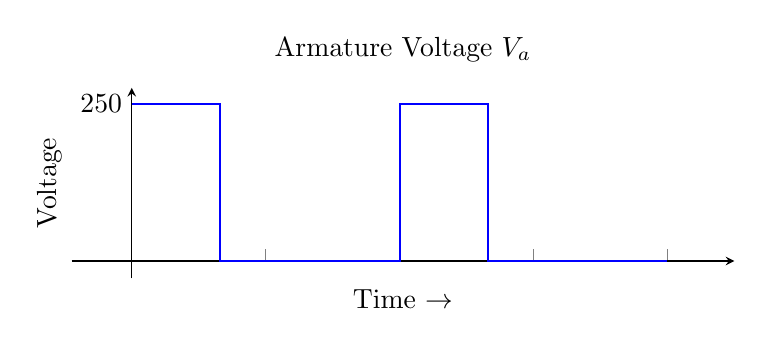
\begin{tikzpicture}
    \begin{axis}[
    width=10cm,
    height=4cm,
    x axis line style={-stealth},
    y axis line style={-stealth},
    title={Armature Voltage $V_a$},
    xticklabels={},
    ymax = 275, xmax=4.5,
    axis lines*=center,
    ytick={0,250},
    xlabel={Time $\rightarrow$},
    ylabel={Voltage}]
    \addplot+[thick,mark=none,const plot]
    coordinates
    {(0,250) (0.66,250) (0.66,0) (2,0) (2,250) (2.66,250) (2.66,0) (4,0)};
    \end{axis}
    \end{tikzpicture}
\end{center}
\begin{center}
    \begin{tikzpicture}
    \begin{axis}[
    width=10cm,
    height=4cm,
    x axis line style={-stealth},
    y axis line style={-stealth},
    title={Back-EMF $e_a$ },
    xticklabels={},
    ymax = 100, xmax=4.5,
    axis lines*=center,
    ytick={0, 75.398},
    xlabel={Time $\rightarrow$},
    ylabel={Voltage}]
    \addplot+[thick,mark=none,const plot]
    coordinates
    {(0,0) (0,75.398) (2, 75.398) (4, 75.398)};
    \end{axis}
    \end{tikzpicture}
\end{center}
Note ignore the vertical up rise on the graph and treat as a constant function throughout. Issues with formatting are the only reason it's there above.
\begin{center}
    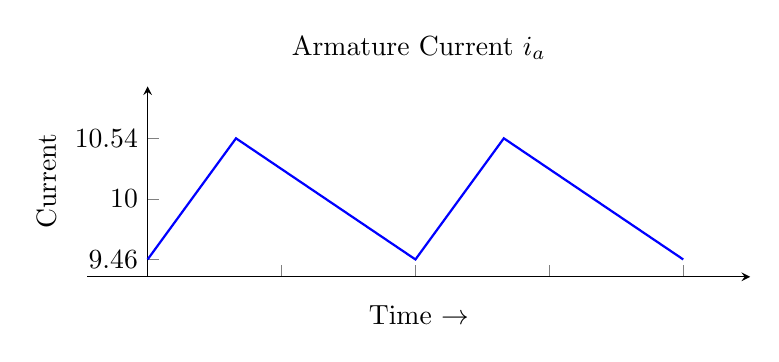
\begin{tikzpicture}
    \begin{axis}[
    width=10cm,
    height=4cm,
    x axis line style={-stealth},
    y axis line style={-stealth},
    title={Armature Current $i_a$},
    xticklabels={},
    ymax = 11, xmax=4.5,
    axis lines*=center,
    ytick={0,9.46187, 10, 10.5381},
    xlabel={Time $\rightarrow$},
    ylabel={Current}]
    \addplot+[thick,mark=none,]
    coordinates
    {(0,9.46187) (0.66,10.5381) (2,9.46187) (2.66,10.5381) (4,9.46187)};
    \end{axis}
    \end{tikzpicture}
\end{center}
\begin{center}
    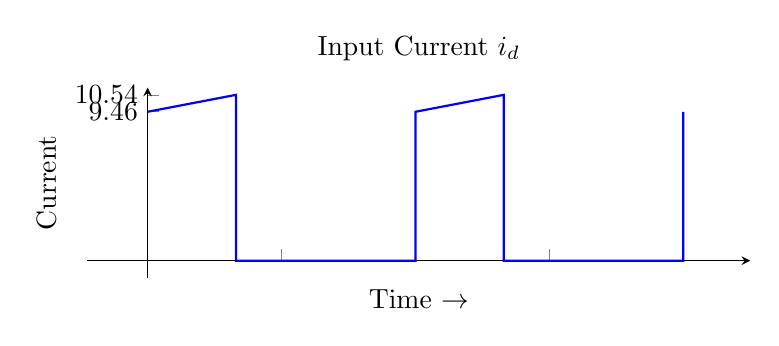
\begin{tikzpicture}
    \begin{axis}[
    width=10cm,
    height=4cm,
    x axis line style={-stealth},
    y axis line style={-stealth},
    title={Input Current $i_d$},
    xticklabels={},
    ymax = 11, xmax=4.5,
    axis lines*=center,
    ytick={0,9.46187, 10.5381},
    xlabel={Time $\rightarrow$},
    ylabel={Current}]
    \addplot+[thick,mark=none,]
    coordinates
    {(0,9.46187) (0.66,10.5381) (0.66, 0) (2,0) (2,9.46187) (2.66,10.5381) (2.66,0) (4,0) (4,9.46187)};
    \end{axis}
    \end{tikzpicture}
\end{center}
\begin{center}
    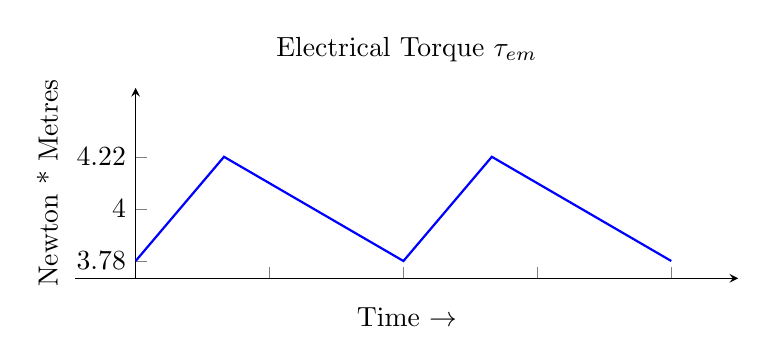
\begin{tikzpicture}
    \begin{axis}[
    width=10cm,
    height=4cm,
    x axis line style={-stealth},
    y axis line style={-stealth},
    title={Electrical Torque $\tau_{em}$},
    xticklabels={},
    ymax = 4.5, xmax=4.5,
    axis lines*=center,
    ytick={0,3.78475, 4, 4.21525},
    xlabel={Time $\rightarrow$},
    ylabel={Newton * Metres}]
    \addplot+[thick,mark=none,]
    coordinates
    {(0,3.78475) (0.66,4.21525) (2,3.78475) (2.66,4.21525) (4,3.78475)};
    \end{axis}
    \end{tikzpicture}
\end{center}

\section*{Part d:}
Simulate the scenarios in points a to c in PSIM and compare results with the calculations. Include relevant waveforms and plots obtained from the simulation.\\ \\
The plots for each corresponding scenario will be seen below on the next page. Of the results we can see that they are all virtually identical to the results obtained in our theoretical calculations. One thing to note is that the speed and torque characteristic was not plotted precisely the same as in part a because this would require many recordings at different speeds so we could build a profile (graphical relationship) between the two for each voltage. However, in the set points it was seen that the points do lie on our characteristic derived in part a. Further I also tested for other speeds but did not include them all since the results proved that the characteristics were accurate as the points all lied on their corresponding curves.
\begin{figure}[H]
    \centering
    \includegraphics[width=0.9\textwidth]{q1-d-120.png}
    \includegraphics[width=0.9\textwidth]{q1-d-75.png}
    \includegraphics[width=0.9\textwidth]{q1-d-45.png}
    \caption{Plots corresponding to the armature voltage of part a}
\end{figure}
\begin{figure}[H]
    \centering
    \includegraphics[width=0.9\textwidth]{q1-d-b.png}
    \caption{Plot corresponding to the armature voltage of part b}
\end{figure}
\begin{figure}[H]
    \centering
    \includegraphics[width=0.9\textwidth]{q1-d.png}
    \includegraphics[width=0.9\textwidth]{q1-d2.png}
    \caption{Plots from running the provided circuit adjusted for our own parameters related to part c}
\end{figure}

\section{Question 2}
A three phase induction motor with the parameters in the table below is connected in Y configuration to a 50Hz source with 440V per phase:
\begin{center}
 \begin{tabular}{| c | c | c |} 
 \hline
 $R_1 = 82m \Omega$ & $X_{l1} = 19 m\Omega$ & $R_2 = 70m\Omega$\\ 
 \hline
 $X_{l2} = 18m\Omega$ & $X_m = 7.2 \Omega$ & No. Poles = 6 \\ 
 \hline
 $P_{losses-mech} = 1.3kW$ & $P_{losses-core} = 1.4kW$ & $P_{losses-misc} = 0kW$\\
 \hline
\end{tabular}
\end{center}
For a slip of 0.04 determine:
\begin{itemize}
    a) The phase current, and copper losses at the armature\\
    b) The air-gap power, and the power converted to mechanical\\
    c) Induced and load torque\\
    d) The overall motor efficiency\\
    e) The motor speed in RPM and rad/sec
\end{itemize}
% \section{Question 2}
\section*{Part a:}
First we must calculate $Z_{eq}$ for the equivalent circuit below:
\begin{figure}[H]
    \centering
    \includegraphics[width=0.7\textwidth]{q2-1.png}
    \caption{Question 2 equivalent circuit}
\end{figure}
Thus we know that $I = \frac{V}{Z_{eq}}$.
\begin{align*}
    Z_{eq} &= (R_1 + X_{l1}) + ( X_m || (R_2/s + X_{l2}) \\
    Z_{eq} &= (R_1 + X_{l1}) + \frac{(X_m) (R_2/s + X_{l2})}{(X_m) + (R_2/s + X_{l2})}\\
    Z_{eq} &= (82*10^{-3} + j*(19*10^{-3}) + \frac{(j*7.2)*((70*10^{-3})/0.04 + (j*18*10^{-3}))}{(j*7.2) + ((70*10^{-3})/0.04 + (j*18*10^{-3}))}\\
    Z_{eq} &= 1.7266 + j(0.43569)
\end{align*}
Moreover, the phase current is: 
\begin{align*}
    I_{phase} &= V_{phase} / Z_{eq}\\
    I_{phase} &= \frac{440}{1.7266 + j(0.43569)}\\
    I_{phase} &= 247.09 \phase{-14.16^{\circ}} [A]
\end{align*}

Moreover the stator copper losses, per-phases are:
\begin{align*}
    P_{Cu-Losses-stator} &= (I_{phase})^2 * R_1 \\
    &= 247.09^2 * 82*10^{-3}\\
    &= 5006.38 [W] = 5.01 [kW]\\
    P_{total-Cu-Losses} &= 3 * P_{Cu-Losses-stator} \\
    P_{total-Cu-Losses} &= 15.03 [kW]
\end{align*}
\section*{Part b:}

To calaculate the air gape power $P_{ag}$ we can use:
\begin{align*}
    P_{ag} &= 3 * \frac{(i_r)^2* R_r}{s}\\
    \longrightarrow &\mbox{ Now we must find $i_r$}\\
    i_r &= \frac{V_{th}}{(Z_{th} + Z_r)} \\
\end{align*}
Find $V_{th}$ and $Z_{th}$\\
\begin{align*}
    V_{th} &= V_s * \frac{Z_m}{Z_s + Z_m}\\
    &= 440 * \frac{j(7.2)}{((82*10^{-3})+j(19.1*10^{-3}))+j(7.2)}\\
    &= 438.808 \phase{-0.651^{\circ}} [A]\\
    Z_{th} &= j * (X_m) || (R_1 + j * X_1)\\
    &= \frac{[j X_m][R_1+jX_1]}{[j X_m]+ [R_1 + jX_1]}\\
    &= \frac{[j(7.2)]*[82*10^{-3} + j(19*10^{-3})]}{[j(7.2)]+[82*10^{-3} + j(19*10^{-3})]}\\
    &= 0.08155 + j (0.019876)\\
    Z_r &= R_2 + X_{l2} + R_2(1/s-1) \\
    &= R_2/s + X_{l2} \\
    &= (70 * 10^{-3})/0.04 + j(18*10^{-3})\\
    &= 1.75+ j(18*10^{-3})
\end{align*}
Finally substituting these values we can calculate the air gap power:
\begin{align*}
    I_r &= \frac{V_{th}}{(Z_{th} + Z_r} \\
    &= 3 * \frac{438.808 \phase{-0.651^{\circ}}}{(0.08155 + j (0.019876))+(1.75+ j(18*10^{-3}))}\\
    &= 239.53 \phase{-0.5339^{\circ}}\\
    P_{ag} &= 3 * \frac{(239.53)^2* 220*10^{-3}}{0.04}\\
    &= 301.22 [kW]
\end{align*}
Next we can calculate the power converted to mechanical (electro-mechanical power) by:
\begin{align*}
    P_{em} &= P_{ag} - P_r \\
    \Longrightarrow \eta_{EM} &= \frac{P_{em}}{P_{ag}} = \frac{(1/s-1}{1/s} = (1-s)\\
    P_{em} &= P_{ag} * \eta_{EM} \\
    &= 301.22 * (1-0.04) \\
    &=289.17 [kW]
\end{align*}
\section*{Part c:}
To calculate induced torque (and load) we first need to find the speeds:
\begin{align*}
    \eta_s &= 120 * f_e / (No. poles) \\
    &= \frac{120*50}{6}\\
    &= 1000 [rpm]\\
    \omega_s &= 104.72 [rad/s]\\
\end{align*}
The induced torque $\tau_{ind}$ 
\begin{align*}
    \tau_{ind} &= \frac{P_{ag}}{\omega_s}\\
    &= \frac{301.22}{104.72}\\
    &= 2.876 [kN*m]\\
    \tau_{load} &= \frac{P_{out}}{\omega_r}\\
\end{align*}
Load torque $\tau_{load}$ we need to find $P_{out}$ and $\omega_r$\\
\begin{align*}
    P_{out} &= P_{in} - P_{Cu-stator-loss} - P_{core-loss} -P_{Cu-rotor-loss} - P_{mech-loss} \\ 
    &= 3*V_s*i_s*cos(\theta_i) - 15.03 - 1.4 - (P_{ag} - P_{em}) - 1.3\\
    &= 3*440*247.09*cos(-14.16^{\circ})-15.03 - 1.4 - (301.22 - 289.17) - 1.3\\
    &= 286.469 [kW]\\
    \omega_r &= \omega_s (1-s) \\
    \tau_{load} &= \frac{286.469}{104.72(1-0.04)}
\end{align*}
Moreover:
\begin{align*}
    \tau_{ind} &= 2876.43 [N*m]\\
    \tau_{load} &= 2849.55 [N*m]
\end{align*}
\section*{Part d:}
To calculate the motor effiency we need the input and output power:
\begin{align*}
    \eta_{motor} &= \frac{P_{out}}{P_{in}}*100\%\\
    &= \frac{286.469}{3*440*247.09*cos(-14.16^{\circ})}*100\%\\
    &= 90.58\%
\end{align*}
\section*{Part e:}
These were previously calculated earlier in the question:
\begin{align*}
    N_s &= 1000 [rpm]\\
    \omega_r &= 100.53 [rad/s]
\end{align*}

\end{document}